%
\documentclass{article}
\usepackage[utf8]{inputenc}

%>>>>>>>>>> AAAI format

\usepackage{aaai20}
\usepackage{times}
\usepackage{helvet}
\usepackage{courier}
\usepackage[hyphens]{url}
\usepackage{graphicx}
\urlstyle{rm}
\def\UrlFont{\rm}
\usepackage{graphicx}
\frenchspacing
\setlength{\pdfpagewidth}{8.5in}
\setlength{\pdfpageheight}{11in}
% Add additional packages here, but check
% the list of disallowed packages
% (including, but not limited to
% authblk, caption, CJK, float, fullpage, geometry,
% hyperref, layout, nameref, natbib, savetrees,
% setspace, titlesec, tocbibind, ulem)
% and illegal commands provided in the
% common formatting errors document
% included in the Author Kit before doing so.
%
% PDFINFO
% You are required to complete the following
% for pass-through to the PDF.
% No LaTeX commands of any kind may be
% entered. The parentheses and spaces
% are an integral part of the
% pdfinfo script and must not be removed.
%
%\pdfinfo{
%/Title (Type Your Paper Title Here in Mixed Case)
%/Author (John Doe, Jane Doe)
%/Keywords (Input your keywords in this optional area)
%}
%
% Section Numbers
% Uncomment if you want to use section numbers
% and change the 0 to a 1 or 2
% \setcounter{secnumdepth}{0}

% Title and Author Information Must Immediately Follow
% the pdfinfo within the preamble
%
\title{An Answer Set Programming Framework for Reasoning about Truthfulness of Statements by Agents} %\\
\author{Marcello Balduccini\\
Saint Joseph's University\\
\And
Michael Gelfond\\
Texas Tech University\\
\And
Enrico Pontelli \ and Tran Cao Son\\
New Mexico State University
} %\\

%<<<<<<<<<< AAAI format




\usepackage{mathptmx}

\usepackage{amsfonts, amsmath, amssymb, mathrsfs}
\usepackage{times, helvet, courier}
\usepackage{graphicx, epsfig, epstopdf}
\usepackage{wrapfig, caption, multirow, url}
\usepackage[ruled,linesnumbered,noresetcount,vlined]{algorithm2e}
\usepackage{stmaryrd}
\usepackage{url}
%\usepackage{alltt}
\usepackage{color}
\usepackage{picinpar}
 
\newboolean{includeMemo}
\setboolean{includeMemo}{true} % boolvar=true or false

%%%%%%\usepackage{tikz}
%%%%%%\usetikzlibrary{arrows,chains,positioning,automata,decorations,shapes,calc,matrix,fit}
%\usepackage{smartdiagram}

%\usepackage[nodisplayskipstretch]{setspace}
%\setstretch{1}

\setlength{\belowdisplayskip}{0pt} 
\setlength{\belowdisplayshortskip}{0pt}
\setlength{\abovedisplayskip}{0pt} 
\setlength{\abovedisplayshortskip}{0pt}


\setlength{\abovecaptionskip}{1pt} 
\setlength{\belowcaptionskip}{-1pt} 

\setlength{\dbltextfloatsep}{-1pt}  
\setlength{\dblfloatsep}{-1pt}

\newcommand{\memo}[1]{
  \ifthenelse {\boolean{includeMemo}}{\medskip\noindent\fbox{\begin{minipage}[b]{\dimexpr\linewidth-1em}#1\end{minipage}}\medskip\newline} 
}
 


\newtheorem{theorem}{Theorem}
\newtheorem{corollary}[theorem]{Corollary}
\newtheorem{lemma}[theorem]{Lemma}
\newtheorem{proposition}[theorem]{Proposition}
\newtheorem{claim}[theorem]{Claim}

\newtheorem{example}{Example}%[section]
\newtheorem{exercise}{Exercise}
\newtheorem{definition}{Definition}
\newtheorem{remark}{Remark}


\def\naf{\: {not} \:}
\def\cra{\stackrel{_+}{\leftarrow}}
\def\executable{\:\: \texttt{executable if} \:\:}
\newcommand{\causesif}[1]{\:\: \texttt{causes} \:\: {#1} \:\: \texttt{if} \:\:}
\newcommand{\ifthen}{\:\:\texttt{if} \:\:}



%\jdate{April 2016}
%\pubyear{2016}
%\pagerange{\pageref{firstpage}--\pageref{lastpage}}
%\doi{S1471068401001193}

 
 
\begin{document}  

\label{firstpage}


\maketitle

\begin{abstract}
The paper proposes a framework for capturing how an agent’s beliefs evolve over time  in response to observations and for answering the question of whether  statements 
made by a third party can be believed. The basic components of the framework are a formalism for 
reasoning about actions, changes, and observations and a formalism for default reasoning. 
The paper describes a concrete implementation that leverages answer set programming for   
determining the evolution of an agent's ``belief state'', based on observations, knowledge about the effects of actions, and a theory about how these influence an agent's beliefs. 
The beliefs are then used to assess whether statements made by a third party can be accepted as truthful. The paper investigates an application of the 
proposed framework in the detection of
 man-in-the-middle attacks targeting computers and cyber-physical systems. 
Finally, we briefly 
discuss related work   and   possible extensions. 
\end{abstract}

% \begin{keywords}
%        Agents, ASP, Reasoning, Knowledge
%  \end{keywords}


 %
\section{Introduction} 

Artificial Intelligence research, in the area of knowledge-based and intelligent agents, has been progressing at
a rapid pace, making it possible to develop agents that can assist and/or replace humans in 
several tasks. Organizations  use  web-bots for interacting with clients in various capacities, e.g., in providing information about the company or making offers. This trend continues to be fueled by the ubiquitous use of online resources. 
Unfortunately, not every business on the Internet is as 
honest as one would hope. Stories about businesses that cheat people of goods or services, or falsely advertise their services are not uncommon. Indeed, lying and misrepresentations are more widespread in online negotiations than 
offline ones \cite{elie}. This concern is also reflected in the 
development of resources that allow people to rate companies (e.g., \url{expedia.com}, \url{yelp.com},  \emph{Angie's List}) or defend the reputation of a company or an entity (e.g., \url{reputation.com}). Dishonesty is also present in
the news media, leading to the dissemination of untruthful stories  (e.g., the `Phuc Dat Bich' story\footnote{ 
{\tiny
\url{http://gizmodo.com/phuc-dat-bich-is-a-massive-phucking-faker-1744588099}
}} reported by BBC and Sky News). Another example is the case of a hotel reviewer with the alias {\em ``AmishBoy''} who gave high ratings to different hotels in the same day \cite{MinnichCMLF15}---thus suggesting  that his statements may be untrustworthy. These situations highlight the problem of  \emph{understanding whether 
statements made by an agent can be accepted as truthful wth respect to a context composed of observations,
knowledge about default behavior, and corresponding beliefs. }


%\begin{example}
%The Gizmodo website carried the following story:\footnote{ 
%{\tiny
%\url{http://gizmodo.com/phuc-dat-bich-is-a-massive-phucking-faker-}\\
%\url{1744588099}
%}}
%A man named Tin Le from Australia managed to fool the world's media by posting his screenshot of a passport with the name ``Phuc Dat Bich'' and claiming that he was denied access to a social network because of his name. It turned out to be a hoax. Yet, before he acknowledged that it was a hoax, BBC and Sky News  reported the story as true. 
%Observe that the story was reported as a true story  even if requests for interview had been denied. 
%\end{example} 
%


%The above example displays a typical situation in which a piece of information is disseminated as true but later found  to be false. It would have been better if the media had verified the truthfulness of the statement before disseminating it. In fact, if they had  applied some common-sense, by considering that  ``{\em normally, a statement cannot be considered as true if it is not verified}'',  then they would  have not reported the hoax. The example suggests the need to develop systems capable of determining whether  a given statement is truthful or not. 




In this paper, we are interested in reasoning about the ``belief state'' of an agent and what that tells us about the truthfulness of statements made by a third party. We assume that we can observe the world as well as other agents' actions. The basis for our judgments will be composed of our observations, performed on
a linear time line, along with  commonsense knowledge about the world and about how observations and knowledge influence an agent's beliefs. We assume that observations are \emph{true} at the time they are made, and will stay true until additional pieces of information prove otherwise. The approach is designed to reflect the fact that an agent's beliefs are subjective -- they might not correspond to the ground truth and could change over time. This is because judgments are often made in the presence of incomplete information. This makes reasoning about beliefs and truthfulness of statements \emph{non-monotonic}. Note that, in this paper, judgments about a statement are made  \emph{independently} of whether or not we trust the agent from whom the statement originated. As such, our study in this paper differs from the 
extensive literature about trust models between agents  (see, e.g., \cite{ArtzG07,SabaterS05}). We will elaborate further on this issue in the related work section. 

\begin{example} \label{ex1}
When we first met at an event (time $t_0$), John stated that he comes from a poor family. 
We later learn that John attends a private college, renowned for  its expensive tuition (time $t_1$). Later on, we learn 
that John attends the college thanks to a  scholarship awarded  due to his financial hardship (time $t_2$).

This story spans over three time instances: $t_0$, $t_1$, and $t_2$. During the story, we learn (through observations) some facts, which  affect our beliefs about the world as follows:    

\begin{list}{$\bullet$}{\itemsep=0pt \topsep=0pt \parsep=0pt \leftmargin=10pt}  
\item Time $t_0$: John makes the statement that his family is poor (property $poor$ is true). No observations are available to us and thus we do not know if John's family is indeed poor or not. We have no reasons to conclude that John's statement is not truthful. 

\item Time $t_1$:  We observe that John attends an expensive college (property $in\_college$ is true). {\emph{Normally}, we believe that someone attending an expensive college is from a rich family.} (default $d_1$). Hence, our belief at this point is that John is rich. This prevents us from accepting John's statement as truthful. We indicate that  the default $d_1$ is the reason to draw such conclusion. 

\item Time $t_2$: We observe that John has a need-based scholarship   (property $has\_scholarship$ is true). {It is our belief that a student's need-based scholarship is \emph{usually} derived from the family's financial situation} (default $d_2$). Because both defaults are applicable and in conflict with each other, we neither believe that John's family is rich, nor that it is poor. This allows us to withdraw our previous conclusion that John's statement could not be accepted as truthful.  

\item The situation might be different if we had a preference between our defaults. For instance, if we were inclined to favor $d_2$ over $d_1$, then we would believe that John's family is poor. This may strengthen our conclusion that John's statement can be accepted as truthful. 
% 
\end{list} 
\end{example}  
The main contributions of this paper can be summarized as follows:
\begin{enumerate}
\item The formalization of an abstract model to 
represent and reason about the evolution of an agent's beliefs over time and to draw conclusions about whether third-party statements can be accepted as truthful; 
\item A concrete realization of the model using
Answer Set Programming; 
\item A use case of the proposed framework on an important problem in the
        area of  cyber security. 
\end{enumerate}
%The paper illustrates  how, starting
% from ({\em (i)}) a collection of observations about the (possibly evolving) state of the
% world, {\em (ii)}
% observations about (some of) the  actions performed by the agent, and 
%{\em (iii)}
% the observer's own bias about the \emph{normal} behavior of agents,
% an observer can draw conclusions about the truthfulness of statements made by
% the observed agent. 
 We illustrate the framework 
 using examples and discuss possible extensions that need to be considered. 
%We also discuss a potential application of the proposed framework. 
 


 \iffalse 



For a rule $r$ of form (\ref{lprule1}), $H(r)$ and 
$B(r)$ denote the left and right hand side 
of $\leftarrow$, respectively; 
$head(r)$ denotes $\{c_1, \ldots,  c_k\}$; and 
$pos(r)$ and $neg(r)$ denote $\{a_1,\ldots,a_m\}$ and 
$\{a_{m+1},\ldots, a_n\}$.  
For a program $\Pi$, $lit(\Pi)$ denotes the set of literals occurring in $\Pi$. 

Consider a set of ground literals $X$. 
$X$ is \emph{consistent} if there exists no atom $a$ such that 
both $a$ and $\neg a$ belong to $X$. The
body of a rule $r$ of the form (\ref{lprule1}) is
{\em satisfied} by $X$ if $neg(r) \cap X = \emptyset$
and $pos(r) \subseteq X$. A rule of form
(\ref{lprule1}) with nonempty head 
is satisfied by $X$ if either its body is not
satisfied by $X$ or $head(r) \cap X \ne \emptyset$. 
A constraint is {\em satisfied} by $X$ 
if its body is not satisfied by $X$. 

For a consistent set of ground literals $S$ and a 
program $\Pi$, the {\em reduct} 
of $\Pi$ w.r.t. $S$, denoted by $\Pi^S$, is the program
obtained from  $\Pi$ by deleting
{\bf (i)} each rule that has a naf-literal {\em not} $a$ in its body with
$a \in S$, and
{\bf {ii}} all naf-literals in the bodies of the remaining rules.

$S$ is an \emph{answer set (or a stable model)} of $\Pi$ \cite{GelfondL90} if it
satisfies the following conditions: 
{\bf (i)}  If $\Pi$ does not contain any naf-literal
(i.e., $m=n$ in every rule of $\Pi$) then $S$ is a minimal 
consistent set of literals that satisfies all the rules in $\Pi$; and
{\bf (ii)} If $\Pi$ does contain some naf-literal
($m < n$ in some rules of $\Pi$), then $S$ is an answer set of
$\Pi$ if $S$ is the answer set of $\Pi^S$. Note that $\Pi^S$ does
not contain naf-literals; hence its answer set is defined in the first
item.
A program $\Pi$ is said to be \emph{consistent} if it has an
 answer set. Otherwise, it is inconsistent. 


To increase the expressiveness of ASP and  
simplify its use in applications, the language
 has been extended with several constructs such as 
\begin{itemize} 
\item Weight constraint atoms (e.g., \cite{nie99b})
of the form: 
%%
\begin{equation}
\label{weight}
\begin{array}{l}
  l\: [a_1 = w_1, \ldots, a_n = w_n, \\
  \hspace*{.4in}{\naf} b_{n+1} = w_{n+1},\ldots,b_{n+k} = w_{n+k} ]\: u 
\end{array}
\end{equation}
%
where $a_i$ and $b_j$ are literals and $l$, $u$, and $w_j$'s are integers,
$l \le u$. 
%Such an atom is satisfied in a set of literal $X$ 
%if $l \le \sum_{a_i \in X} w_i + \sum_{b_{n+k} \not\in X} w_{n+k} \le u$. 
 

\item Aggregates atoms (e.g, \cite{faberLP04,PelovDB04,SonP05})
 of the form:
%%
\begin{equation}
\label{weight}
f(S) \: op \: v
\end{equation} 
where $S$ is a set-literal, $f \in \{\textnormal{\sc Sum}, \textnormal{\sc Count},
\textnormal{\sc Max}, \textnormal{\sc Min} \}$, 
$op \in \{>, <, \ge, \le, =\}$, 
and $v$ is a number; a set-literal is of the form   
({\em i}) $\{\vec{X} \mid p(\vec{W})\}$ where $\vec{X}$ is a vector of variables, $\vec{W}$ is vector of parameters and constants such that each variable in $\vec{X}$ also occurs in $\vec{W}$; 
or ({\em ii}) $\{\!\!\{\vec{X} \mid \vec{Y}. p(\vec{W})\}\!\!\}$ where $\vec{X}$ and $\vec{Y}$ are vectors of variables, $\vec{W}$ is vector of parameters and constants such that each variable in $\vec{X}$ or $\vec{Y}$ also occurs in $\vec{W}$.

\end{itemize}  
 %
The semantics of logic programs with such atoms has been defined  (e.g., \cite{faberLP04,nie99b,PelovDB04,SonP05}. Standard syntax for these types of atoms has been proposed and adopted in most state-of-the-art ASP-solvers such as 
\textsc{clasp}~\cite{GebserKNS07} and \textsc{dlv}~\cite{dlv97}. 

\subsection{Action Languages}
\emph{Action languages} \cite{gl98,causal2} are logic-based languages
used to describe actions and their direct and indirect effects. In the rest
of this section, we will concentrate on the action language $\cal B$.

The language of $\cal B$ is based on a signature ${\cal K} = ({\cal L}, {\cal A})$, where
$\cal L$ is a set of ground atoms, referred to as \emph{fluents},
 and $\cal A$ is a set of \emph{action names}. A fluent literal is a literal
 built on $\cal L$.
 A domain description of $\cal L$ is composed of a collection of \emph{axioms} of 
 the following types:
 \begin{list}{$\bullet$}{\topsep=1pt \itemsep=1pt \parsep=0pt \leftmargin=10pt}
 \item \emph{Executability Axioms:} these describe the conditions that enable the
         execution of an action, and they have the form $a \executable \ell_1\wedge \dots\wedge \ell_n$,
         where $a\in {\cal A}$ and $\ell_1,\dots,\ell_n$ are fluent literals.
  \item \emph{Dynamic Causal Laws:} these descriptions the direct effects of the execution
          of an action, and they have the form
          $a \causesif{\ell} \ell_1\wedge \dots \wedge \ell_n$
          where $a\in {\cal A}$ and $\ell,\ell_1,\dots,\ell_n$ are fluent literals.
  \item \emph{Static Causal Laws:} these description static dependencies among fluents, and they
          have the form
          $\ell \ifthen \ell_1\wedge\dots\wedge\ell_n$
          where $\ell, \ell_1,\dots,\ell_n$ are fluent literals.
 \end{list}
 A planning problem in $\cal K$ is a tuple $(D, I, O)$, where $D$ is a domain description
 of $\cal K$ and $I, O$ are two consistent sets of fluent literals---denoting, respectively,
 the initial state and the goals of the planning problem.

The semantics of $\cal B$ is based on the definition of transition functions. A set of fluent
literals $S$ 
is consistent and complete if for each $f \in {\cal L}$ we 
have that $\{f,\neg f\}\cap S \neq \emptyset$ and $\{f,\neg f\} \not\subseteq S$. A
set of literals $S$ is closed if, for each static causal law $\ell \ifthen \ell_1\wedge\dots\wedge \ell_n$,
if $\{\ell_1,\dots,\ell_n\}\subseteq S$ then $\ell\in S$. The closure $Cn(S)$ of $S$ is the 
smallest set of fluent literals that contains $S$ and is closed. The states are the complete
and closed set of fluent literals of $\cal L$. 

A domain description defines a transition system $(S,a,S')$, where $a\in {\cal A}$, $S,S'$ are
states, and $S' = Cn((S \cap S') \cup X)$, where $X$ is the set of literals $\ell$ such that
there is a dynamic causal law $a \causesif{\ell} \ell_1\wedge \dots \wedge \ell_n$ and
$\ell_1,\dots,\ell_n \in S$. A trajectory for a planning problem $(D,I,O)$ is a 
sequence $S_0 a_0 S_1 a_1 \dots S_n$ such that $(S_i,a_i,S_{i+1})$ is a transition for
$0\leq i <n$, $I \subseteq S_0$, and $O \subseteq S_n$. A sequence of actions $a_0 \dots a_{n-1}$ is
a plan if there is a trajectory $S_0 a_0 \dots a_{n-1}S_n$.
\fi
%


\section{Beliefs and Truthfulness of Statements} 

In this section, we propose a general framework for representing, and reasoning about, the beliefs held by an agent. The framework also establishes a link between the beliefs held by the agent and whether it can accept as truthful statements made by a third party. The
framework  can be instantiated using specific paradigms for reasoning about actions and change and for non-monotonic reasoning. We make
the following assumptions:
%
 \begin{itemize}
%
\item It is possible to  observe the properties of the world and the occurrences of the actions    over time
        (e.g., we observe that John buys a car, John is a student, etc.). Let us denote with $O_a$ and $O_w$ 
        the set of action occurrences and the set of observations about the world over time, respectively. 

\item We have adequate knowledge about actions  and their effects (e.g., the action of buying a car requires that the agent has money and its execution will result in the agent owning a car). This knowledge is represented by an action theory $Act$ in a suitable logic $A$ that allows  reasoning about actions' effects and consequent changes to the world. Let us denote with $\models_A$ the entailment relation defined within the logical framework $A$ used to describe $Act$.    

\item We have commonsense knowledge about how an agent of interest forms its beliefs (e.g., an agent may believe that a person attending an expensive school normally comes from a rich family, a person obtaining need-based scholarship s  usually comes from a poor family).
This knowledge is represented by a default theory with preferences $\textit{Def}$,  that enables reasoning about the state of the agent's beliefs. Let us denote with $\models_D$ the entailment relation defined over the default theory framework defining $\textit{Def}$.  
 
\end{itemize} 

The set of observations $O_w$ in Example~\ref{ex1} includes the observations such as 
%`John comes from a poor family' at time point $t_0$, 
`John attends an expensive college' at time point $t_1$, and `John receives a need-based scholarship' at time point $t_2$. In this particular example we do not have any  action occurrences, i.e., $O_a = \emptyset$.\footnote{Some frameworks for reasoning about actions and change may require the introduction of a NOP action for modeling the example.} Our default theory $D$ consists of defaults $d_1$ and $d_2$ stated earlier, which allow us to make conclusions regarding our agent's beliefs. 

%TEMP
\begin{figwindow}[1,r,%
        {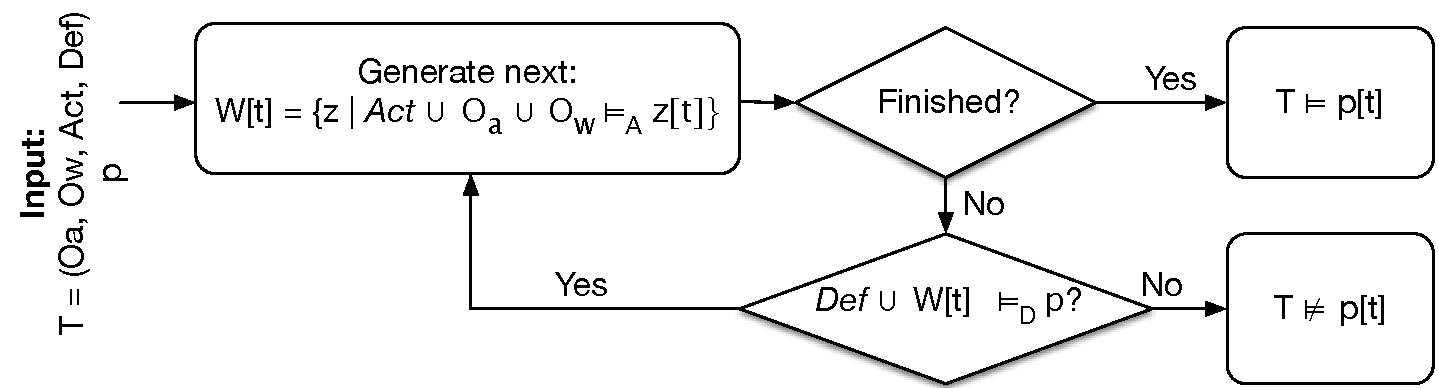
\includegraphics[width=0.48\textwidth]{newstep.pdf}},%
        {Answering Question: $(O_a,O_w,Act,Def) \models p[t]$?\label{fig:schema} }]
\end{figwindow}
Let us consider a theory $T = (O_a, O_w, Act, \textit{Def})$ and the associated entailment relations $\models_A$ and $\models_D$. First and foremost, we are interested in defining the beliefs held by the agent over time. And, then, we are interested in using this information for answering the question of whether a statement $p[t]$,  made at time step $t$ about a proposition $p$, can be accepted as truthful. For this, we define the entailment relation $\models$ between $T$ and $p[t]$. Intuitively, the process entails the steps below (Figure~\ref{fig:schema}):
\begin{list}{$\bullet$}{\itemsep=0pt \parsep=0pt \topsep=0pt \leftmargin=8pt} 
\item Compute possible models $W[t]$ of the world  at the time step $t$ from  $Act$, $O_a$, and $O_w$ (using $\models_A$); and  
\item Determine  the agent's beliefs by finding which propositions are true  given  $\textit{Def}$ and $W[t]$ (using $\models_D$); \textbf{CHECK FOR ISSUES DUE TO THINGS THAT ARE *TRUE* FROM W[t]}
\item Determine if the statement $p[t]$ is consistent with respect to the agent's beliefs. 
\end{list} 
%
Let us assume that the equation $W[t] = \{z \mid Act \cup O_a \cup O_w \models_A z[t]\}$ characterizes
any of the states of the world  at  time step $t$ given $Act$, $O_a$, and $O_w$ (based on the semantics of 
$\models_A$). The entailment relation between $T$ and $p[t]$ can be defined as follows.
%
{\begin{equation} \label{entail} 
T \models p[t] \Leftrightarrow
\begin{array}{c} 
%T \models p[t] \\
% \textit{if and only if} \\
  \forall W[t]. \left(\begin{array}{c}
   W[t] = \{z \mid Act \cup O_a \cup O_w \models_A z[t]\} \Rightarrow \\
                                                                 Def \cup W[t] \models_D p
                                                                \end{array}\right)
\end{array} 
\end{equation} }
%
Note that this definition also allows one to identify elements of $O_a$ and $O_w$ which, when obtained, will result in the 
confirmation or denial of $T \models p[t]$. As such, a system that obeys \eqref{entail} can also be used by users who are 
interested in  what they need to do in order to believe in a statement about $p$ at the time step $t$,
 given their beliefs about the behavior of the observed agents. 


%
%\smartdiagram[flow diagram:horizontal]{Edit,
%  \LaTeX, Bib\TeX/ biber, make\-index, \LaTeX}
\iffalse\begin{figure}
\centering
\resizebox{1.6in}{!}{% 
\smartdiagram[priority descriptive diagram]{
  $W[t]$ model of $A \cup O_a \cup O_w$ restricted to time step $t$,
  $\forall W[t]. (D \cup W[t] \models_D p)$?}
}  
\caption{Answering $(O_a,O_w,A,D) \models p[t]$?}
\label{fig:schema} 
\end{figure} \fi
%
To develop a concrete system for reasoning about truthfulness of agents using \eqref{entail}, specific formalizations of $Act$ and $\textit{Def}$ need to be developed. There is a large body of research related to these two areas, and deciding which one to use depends on the system developer. 
Well-known formalisms for reasoning about actions and change, such as action languages \cite{GelfondL98}, situation calculus \cite{Reiter01}, etc., can be employed for $Act$ (and $\models_A$).  
Approaches to default reasoning with preferences, such as those proposed in  \cite{brew99,BrewkaE00,DelgrandeST03,GelfondS98}), can be used for $\textit{Def}$ (and $\models_D$). In addition, 
let us note that, in the literature, $\models_D$ can represent \emph{skeptical} or \emph{credulous} reasoners; and  the model does not specify how observations are collected. Deciding which type of reasoning is suitable or how to collect observations is an important issue, but it is application-dependent and beyond  the scope of this paper. 
%In this paper, we use observations  in a broad sense: it might be something that we learn some facts about a property of the world, or we actually observed it (via the execution of an action), etc. 
%
\section{Reasoning about Truthfulness of Agents Using Answer Set Programming (ASP)}  

We will now present a concrete system for reasoning about truthfulness of agents using \emph{Answer Set Programming (ASP)}.  We select ASP as the host language since there exist several approaches to reasoning about actions and changes as well as default reasoning using ASP. This enables  the seamless integration of the two steps involved in ~\eqref{entail} into a single system. 
Several efficient ASP solvers are available, that enable the use of the proposed system in practical applications. In particular, we will use answer sets (and projections of answer sets over specific time points) to capture $W[t]$, and use established encodings of action theories and defaults in ASP.
  
 
\subsection{Background: Answer Set Programming}

ASP is a programming paradigm \cite{Niemela99,MarekT99}  based on logic programming under the answer set semantics \cite{GelfondL90}. 
A logic program $\Pi$ is a set of rules of the form 
 $$c  \leftarrow a_1,\ldots,a_m,\naf a_{m+1},\ldots,\naf a_n$$ 
%
where $0 \le m \le n$,   $a_i$'s and $c$ 
are  ground literals in a first order language,\footnote{Rules with variables represent the set of all 
        of their  ground instances.}   
and $\naf$ represents {\em default negation}. 
A rule is satisfied by a set of literals $S$ if $c \in S$, or $\{a_1,\ldots,a_m\} \setminus S \ne \emptyset$, or $\{a_{m+1},\ldots,a_{n}\} \cap S \ne \emptyset$. A consistent set of literals $S$ is a model of a program if it satisfies all the rules of the program. $S$ is an answer set of a program if it is a consistent minimal model of the program obtained by {\em (i)} deleting all rules with some $a \in S$ such that $not \: a$ appears in the rule; and {\em (ii)} deleting all  $not \: a$ from the remaining rules.  Programs without an answer set are said to be inconsistent. Answer sets can be computed using answer set solvers. Extended syntactic notations have been proposed to facilitate the encoding of commonly used patterns (e.g., aggregates). In this paper, we use the  syntax of ASP used in  {\sc Clasp}\footnote{
  \url{http://potassco.sourceforge.net/}
} or Dlv\footnote{\url{http://www.dlvsystem.com/}
}. 




%
%A negation-as-failure literal (or
%naf-literal) is of the form $\naf a$ where $a$ is a literal. For a
%rule of the form (\ref{lprule1}), the left and
%right hand sides of the rule are called the \emph{head} and the
%\emph{body}, respectively. Both the head and the body can be empty. 
%When the head is empty, the rule is called a {\em constraint}. 
%When the body is empty, the rule is called a {\em fact}. 
%


\subsection{Reasoning with No Observations about Action Occurrences}

Let us start with a simpler case---where we do not worry about action
occurrences. Let us assume  a propositional language (i.e., a {\em signature}) $\cal L$, 
whose elements are called fluents. Let us also assume that $\cal L$ does not contain the following predicates: 
$stm$ (for $statement$), $obs$ (for $observed$), $rule$, $default$, and $prefer$. 
Fluent literals (or literals) and (fluent) formulae are defined as usual, using 
propositional combinations of fluents. $\overline{l}$ 
denotes the negation of literal $l$. Agents can make statement about literals.  
Statements are given in the form {$stm(p,s)$}
where  $s$ is a non-negative integer (representing a time step) and $p$ is a literal.  
For example, the statement `John said that he is poor'  can be stated as 
$stm(poor, 0)$. 

%
%\begin{definition} 
%A \emph{statement} about a   literal $p$ is of the form 
%\begin{align}\label{stat}
%stm(p,  s)  
%\end{align} 
%where  $s$ is a non-negative integer. 
%\end{definition} 
%For example, John said that he is poor. This can be stated as 
%$
%stm(poor, 0) 
%$
%says that $poor$ is true at time step 0. 

%Another example is that John said that he is poor. This can be stated as 
%\[
%stm(poor, 0) 
%\]
%states that $poor$ is true at time step 0. 

\iffalse
We can make observations about fluent literals. 
\begin{definition} 
An observation about a fluent literal $P$ is of the form 
\begin{equation}\label{obs}
obs((P,   S)  
\end{equation} 
where  $S$ is a non-negative integer. 
\end{definition} 
Note that $obs$ is understood in a broad sense: it might be that we learn some facts about the fluent literal, or we actually observed it (via the execution of a sensing action), etc. 

For example, if we observe that John is not sick, we use 
\[
obs(\neg sick, 0). 
\]


Our reasoning module consists of a collection of rules and defaults, possibly with priorities among defaults. 
\begin{itemize} 
\item A \emph{rule} is of the form 
\begin{align}\label{rule}
rule(r, head, body)
\end{align} 
where $r$ is the name of the rule, $head$ is a fluent literal, and $body$ is a collection of literals. A rule \eqref{rule} says that whenever $body$ holds then $head$ must also hold. 
\item A \emph{default} is of the form 
\begin{align}\label{default}
default(d, head, body)
\end{align} 
where $d$ is the name of the default, $head$ (or \emph{conclusion}) is a fluent literal, and $body$ is a collection of literals.  A default \eqref{default} says that, normally, if $body$ holds then $head$ also holds. 
\item A \emph{preference} between two defaults is expressed by 
\begin{align}\label{pref}
prefer(d_1, d_2, body)
\end{align} 
where $body$ is a set of fluent literals and $d_1$ and $d_2$ are names of two defaults. This says that 
the default $d_1$ is  preferred to $d_2$ whenever $body$ holds.

\end{itemize} 

\fi

\begin{definition} 
A \emph{knowledge base (KB)} about an agent, over a signature  $\cal L$, 
is a pair $\langle  O, RD \rangle$ where: 
\begin{list}{$\bullet$}{\topsep=1pt \parsep=0pt \itemsep=1pt \leftmargin=10pt}
\item $O$ is a set of observations, each of the form 
{
\begin{align}\label{obs}
obs(p,  s)  
\end{align} 
}
where $p$ is a literal and $s$ is a non-negative integer; 
\item $RD$ is a collection of expressions of the form 
{
\begin{align}
rule(r, head, body)\label{rule} \\
default(d, head, body) \label{default} \\
prefer(d_1, d_2, body) \label{pref}
\end{align} 
}
where $r$, $d$, $d_1$, and $d_2$ are constants which do not belong to $\cal L$, 
$head$ is a literal and $body$ is a set of literals in $\cal L$.  
\eqref{rule}, \eqref{default}, and \eqref{pref} are referred to as a 
 \emph{rule}, a \emph{default}, and a 
 \emph{preference} between defaults, respectively.  
\end{list} 
\end{definition} 
Intuitively, $r$ and $d$ are used to name rules and defaults. 
%
%We will next define the notion of consistent knowledge bases. 
We say that a set of observations $O$ is \emph{consistent} if, for each time step $s$ and proposition $p$, $\{obs(p,s), obs(\neg p, s)\} \not\subseteq O$. 
A set of rules and defaults $RD$ is \emph{consistent} if, for any consistent set of literals $X$, the logic program 
$\{head \leftarrow body  \mid rule(r, head, body) \in RD\} \cup \{\ell \leftarrow \:\mid\: \ell\in X\}$
is consistent.  
%
\begin{definition}
A $KB = \langle O, RD \rangle$ is \emph{consistent} if $O$ and $RD$ are consistent. 
\end{definition} 
%
Our goal is to identify whether  a statement $stm(p, s)$ is true at a time step $t$ for $t \ge s$ given a $KB$. We will develop a program $\Pi(KB)$ to answer this question. We assume a finite horizon of steps, denoted by $s(0), \ldots, s(k)$. We use $h(P,S)$ to encode that literal $P$ is true at step $S$. Furthermore, to simplify the use of $\Pi(KB)$ with current ASP solvers, we  encode a rule of the form \eqref{rule}  using {\bf (a)} the ASP atom $rule(r, head, name)$ and
{\bf (b)} the set of ASP atoms $\{mem(l, name) \mid l \in body\}$, where \(name\) is a unique identifier for the rule; similar encodings are used for  \eqref{default} and \eqref{pref}. 
This method of encoding is similar to what is used  in answer set planning and allows for the separation between  the encoding of the problem and the rules for reasoning with it.
The main challenge to be addressed lies in the interaction between observations, defaults, etc. 
We apply the following principles:
%
 \begin{list}{$\bullet$}{\topsep=0pt \parsep=0pt \itemsep=0pt \leftmargin=10pt}
\item[]{\bf (O)}ptimistic: The most recent observation reflects the true state of the world;
\item[]{\bf (SK)}eptical: When conflicting conclusions can be drawn then do not believe in any.
\end{list} 
%
$\Pi(KB)$ contains the set of facts encoding $O$ and $RD$ as described above. We next describe the rules in $\Pi(KB)$. 
%
The following rules are used to  reason about observations of the form 
\eqref{obs}:\footnote{The  predicate $neg$ encodes the complement of a literal).}
%
\begin{eqnarray}  
h(P, S)  & \leftarrow &   obs(P,S_1), s(S),  S_1 \le S, \naf nr(P, S_1, S).  \label{lp:obs} \\
%               \naf \:not\_most\_recent(P, S_1, S).  \nonumber \\
% not\_most\_recent(P, S_1, S) \leftarrow s(S_1),  \label{lp:obs1}  \\ 
  nr(P, U, S)  & \leftarrow &  s(U), neg(P,P_1), obs(P_1, V), s(S),  U {<} V, V {<} S.  \label{lp:obs1}  %\\ 
%obs(\overline{P}, S_2), s(S),  S_1 < S_2, S_2 < S. \nonumber
\end{eqnarray} 

These rules encode the principle {\bf (O)}. Rule \eqref{lp:obs1} states that $nr(P,S_1)$ is true if there exists a more recent observation of  $\neg P$. Rule \eqref{lp:obs} indicates that an observation stays true if every conflicting observation is `older'.
 
 For reasoning about rules  of the form \eqref{rule}, we have:  %
{
\begin{equation}\label{lp:rule}
\begin{array}{ll}
h(H, S) \leftarrow & s(S),  rule(D, H, M),  N = \# count \{L : mem(L, M),  h(L, S) \},\\ 
     & N  == \# count \{L : mem(L, M)\}.
      \end{array}
\end{equation} 
}
%
This rule  says that if the body of a rule is satisfied then the head of the rule must be true. 

 For reasoning about defaults  of the form \eqref{default} we have:
%%\iffalse
%{\small
%\begin{align}
%app(D, H, S) & \leftarrow   s(S), default(D, H, M),\label{lp:app} \\
%      &NC  = \# count \{L : mem(L, M)\}, \nonumber \\ 
%     & \# count \{L : mem(L, M),     h(L, T) \} == NC. \nonumber \\ 
%ab(D, H, S)& \leftarrow   s(S), app(D, H, S),\label{lp:ab} \\
%    &  app(D_1, \overline{H}, S),  %\nonumber \\
%      \naf defeated(D_1, \overline{H}, S).  \nonumber      \\
%defeated(D, H, S)& \leftarrow   s(S), app(D, H, S), h(\overline{H}, S).\label{lp:defeat0} \\
%    &  app(D, H, S), % \nonumber \\
%      h(\overline{H}, S). \nonumber \\       
%defeated(D, H, S)& \leftarrow   s(S),  app(D, H, S), \label{lp:defeat} \\
%    & app(D_1, \overline{H}, S), prefer(D_1, D, S).  \nonumber \\
%%      prefer(D_1, D, S).  \nonumber      \\
%%h(l_1, S), \ldots, h(l_k, S), \naf ab(d, l, S)   \label{lp:def}\\
%%b(l, S) \leftarrow b(l_1, S), \ldots, b(l_k, S), \naf ab(d, l, S)   \label{lp:def_bel}\\
%%app(d, l, S) \leftarrow h(l_1, S), \ldots, h(l_k, S) 
%h(H, S)& \leftarrow  app(D, H, S), \naf ab(D, H, S),  \label{lp:holds} \\
% % \naf ab(D, H, S), \nonumber \\ 
% & \naf defeated(D, H, S). \nonumber 
%\end{align} 
%} 
%%\fi
%
{
        \[
        \begin{array}{llr}
     app(D, H, S)  \leftarrow &  s(S), default(D, H, M),  
        NC  = \# count \{L : mem(L, M)\},  & (9)\\ %\label{lp:app}
        & \# count \{L : mem(L, M),     h(L, T) \} == NC.  \\ 
        ab(D, H, S) \leftarrow  & s(S), app(D, H, S), neg(H,H_1), & (10)\\   %\label{lp:ab}
        &  app(D_1, H_1, S),  \naf defeated(D_1, H_1, S).        \\
        defeated(D, H, S) \leftarrow  & s(S), app(D, H, S), neg(H,H_1), h(H_1, S).  \:\:\: & (11) \\ %\label{lp:defeat0} 
        defeated(D, H, S) \leftarrow  & s(S),  app(D, H, S), neg(H,H_1), & (12) \\  %\label{lp:defeat}
        & app(D_1, H_1, S), prefer(D_1, D, S).   \\
        h(H, S) \leftarrow & app(D, H, S), \naf ab(D, H, S), \naf defeated(D, H, S).  & (13) \\ %\label{lp:holds}
        \end{array}
        \]
        }
%
The rule for {\it app} defines when a default is \emph{applicable}, i.e., when its body is satisfied. The interaction between defaults and rules in the knowledge base are dealt with using rules for {\it ab} and {\it defeated}. The first rule
        for {\it defeated}  dismisses the applicability of a default if the complement of its conclusion is already established. The second rule for {\it defeated} expresses that a default is defeated if there is a  preferred default with a conflicting conclusion that is applicable.
The rule for {\it ab} enforces the principle {\bf (SK)}. It states that a default $d$ should be blocked if there is another default with the conflicting conclusion ($\overline{h}$), which is not defeated.
Finally, the last rule  enforces the application of any default that is applicable and not otherwise blocked.
 
 \setcounter{equation}{13}
 
 For reasoning about preferences of the form \eqref{pref}, we employ the rules:
{
\begin{equation}\label{lp:pref}
\begin{array}{ll}
prefer(D_1, D_2, S) \leftarrow &  s(S),   prefer(D_1, D_2, M),   N  = \# count \{L : mem(L, M)\},  \\ 
     & \# count \{L : mem(L, M),  h(L, S) \} {==} N. 
      \end{array}
\end{equation} 
}
This rule defines when a preference among two defaults can be applied. 
%
%\iffalse 
%Rule~\eqref{lp:app} defines when a default is \emph{applicable}, i.e., when its body is satisfied. The interaction between defaults and rules in the knowledge base are dealt with using rules~\eqref{lp:ab}---\eqref{lp:defeat}. Rule~\eqref{lp:ab} enforces the principle {\bf (SK)}. It says $ab(d, h, s)$ that if there is another default with the conflicting conclusion ($\overline{h}$) 
%which is not defeated then $ab(d, h, s)$ is true. This atom will be used to suppress the conclusion of $d$.   
%\eqref{lp:defeat0} dismisses the applicability of a default if the contrary of its conclusion is already established. On the other hand, rule \eqref{lp:defeat} expresses that a default is defeated if there is a more preferred default with conflicting conclusion that is applicable.  
%
%
% 
%
%\item Rules for reasoning about beliefs  
%\begin{align}
%b(L, S) \leftarrow h(L, S)  \label{lp:belief}   
%\end{align} 
%
%
%\item For interacting between defaults, we have the following rules: 
%
%%\memo{
%%}
%
%\begin{center} 
%  \begin{tikzpicture} 
%%    \tikzstyle{every node}=[draw,shape=circle} 
%%    \node (s1) at (0:0) {$\alert{s_3:}$}   
%%      \draw[fill=blue!20,style=dashed] (-1.0,-1.0) rectangle (3.0,3.0)  ;
%
%      \draw (0,0) circle(0.4) node {$\textcolor{red}{\small s{-}1}$} ;
%      \draw  (2,0) circle(0.4) node  {$\textcolor{red}{\small s}$} ;
%     \draw  (4,0) circle(0.4) node {$\textcolor{red}{\small s{+}1}$} ;  
% 
%     \draw[-,style=dashed] (-1.6,0) -- (-0.4,0 )  ; 
%     \draw[-] (0.4,0) -- (1.6,0)  ;  
%     \draw[-] (2.4,0) -- (3.6,0 )  ; 
%     \draw[-,style=dashed] (4.4,0) -- (5.6,0 )  ; 
% 
%  \end{tikzpicture} 
%\end{center} 
%
%
%\begin{align}\label{lp:ab} 
%ab(D_1, L, S) \leftarrow \: \: &     default(D_1, L, Body_1),   \\
%    &      app(D_1, L, S), \nonumber \\
%    &      default(D_2, \overline{L}, Body_2), \nonumber \\
%    &      app(D_2, \overline{L}, S), \nonumber \\
%    &      \naf app(D_2, S-1).  \nonumber
%\end{align} 
%
%This rule encodes the principle {\bf (P3)}. 
%
%\fi
%
%
%
%% We will assume that things behave in accordance to the law of inertia. So, we will add to the the program the rule 
%%
%% \begin{align}
%% h(l, S+1) \leftarrow h(l, S),  \naf h(\overline{l}, S)   \label{lp:inertial} \\
%% b(l, S+1) \leftarrow b(l, S),  \naf b(\overline{l}, S)   \label{lp:inertial_bel} 
%% \end{align} 
%
%

In summary, for a $KB = \langle O, RD \rangle$, $\Pi(KB)$ consists of rules~\eqref{lp:obs}--\eqref{lp:pref} and the set of facts encoding $RD$ and $O$.
%
\begin{example} \label{ex2}  
The story in Example~\ref{ex1} 
can be represented by the $KB_1 = \langle  O_1, RD_1 \rangle$ where 
%$O_1 = \{obs(in\_college, 1), obs(has\_scholarship, 2)\}$ and  
%$RD_1 = \{default(d_1, \neg poor, [in\_college])$,
%$default(d_2, poor, [has\_scholarship])\}$.
%
{
\[
\begin{array}{lll}
O_1 & = & \left\{
\begin{array}{l} 
%stm(poor, 0). \\
obs(in\_college, 1). \\ 
obs(has\_scholarship, 2).
\end{array}
\right \},   \\
 RD_1 & = & \left\{
\begin{array}{l} 
default(d_1, \neg poor, [in\_college]). \\
default(d_2, poor, [has\_scholarship]).  
\end{array}
\right \} 
\end{array} 
\]
}
%
The statement in Example~\ref{ex1} can be represented by  $stm(poor, 0).$ 
Consider   $\Pi(KB_1)$ with $k=0,1,2$:  
%
 \begin{list}{$\bullet$}{\topsep=0pt \parsep=0pt \itemsep=0pt \leftmargin=10pt}
\item   $k=0$: since there is no observation, no answer set of $\Pi(KB_1)$ contains any atom of the form $h(l, 0)$; %where $l$ is a literal.
 
\item   $k=1$: because $obs(in\_college,1)$, $h(in\_college,1)$ is true, 
%% is in every answer set of $\Pi(KB_1)$.  
$d_1$ is applicable but $d_2$ is not.  So, every answer set of $\Pi(KB_1)$ contains    $h(in\_college, 1)$ and $h(\neg poor, 1)$.  

\item   $k=2$: %every answer set of $\Pi(KB_1)$ contains 
$h(has\_scholarship,2)$, $h(in\_college,1)$, and $h(in\_college,2)$ are true and $d_1$ is applicable at 1 and 2; $d_2$ is not applicable at   1 but is applicable at   2.  Hence, every answer set of $\Pi(KB_1)$ contains $h(\neg poor, 1)$.  However, none of the answer set   contains $h(poor, 2)$ or $h(\neg poor, 2)$.  

\end{list} 



% Rules for reasoning about statements of the form \eqref{stat} 
% \begin{align}\label{lp:stat}
% b(p, s) \leftarrow stm(p,s), \naf h(\overline{p},s) 
% \end{align} 
% This rule encodes the principle {\bf (P2)}. 


%
%\begin{verbatim}
%s(0..length).
%
%stm(poor, true, 0).
%obs(attend, 1).
%obs(scholarship, 2).
%
%default(d1, -poor, [attend]). 
%default(d2, poor, [scholarship]).
%
%h(poor,T):- s(T), stm(poor,T), not h(-poor,T).  
%
%h(-poor, T):- s(T), h(attend, T), not ab(attend, -poor, T).        
%
%h(F, T) :- s(T), obs(F, T).                                                 
%
%h(poor, T) :- s(T), h(scholarship, T), not ab(attend, poor, T).
%
%ab(attend, -poor, T) :- s(T), h(scholarship, T).
%
%h(F, T+1) :- fl(F), s(T), T<length, h(F, T), not h(-F, T+1). 
%h(-F, T+1) :- fl(F), s(T), T<length, h(-F, T), not h(F, T+1). 
%
%fl(poor).
%fl(attend).
%fl(scholarship).
%\end{verbatim} 
\end{example} 
 
Given a $KB=\langle O, RD \rangle$ over $\cal L$, 
an integer $k$, and a $stm(l,s)$, we 
are interested in determining the truthfulness of the statement 
at time steps $s \le t \le k$. %This is defined as follows. 

\begin{definition} \label{kb:entail}
Let $KB =  \langle O,RD \rangle$ be a knowledge base. Let $stm(l,s)$ be a statement about a literal $l$ at 
the time step $s$ and $t$ be a time step such that $t \ge s$. We say that 
 \begin{list}{$\bullet$}{\topsep=0pt \parsep=0pt \itemsep=0pt \leftmargin=5pt} 
\item $KB \models {+}stm(l,s)@t$ (or $stm(l, s)$ 
is \emph{true} w.r.t. $KB$ at   $t$)  if  $h(l,t) \in A$ for every answer set $A$ of $\Pi(KB)$; 
\item $KB \models {-}stm(l,s)@t$ (or 
$stm(l, s)$ 
is \emph{false} w.r.t. $KB$  at  $t$)  if  $h(\overline{l},t) \in A$ for every answer set $A$ of $\Pi(KB)$;
\item $KB \not\models {\pm}stm(l,s)@t$ (or 
$stm(l, s)$ 
is \emph{unknown} w.r.t. $KB$  at  $t$)    
if $KB \not\models +stm(l,s)@t$ and $KB \not\models -stm(l,s)@t$.

\end{list} 
\end{definition} 

Intuitively, $KB  \models {+}stm(l,s)@t$ (resp. $KB  \models {-}stm(l,s)@t$) says that at the time step $t$ the statement is true (resp. false). $KB \not\models {\pm}stm(l,s)@t$ states that there is no information that supports or denies the statement at the time step $t$. Observe that $l$, $t$, and $s$ are constants representing the question whether or not $stm(l,s)$ is true at step $t$. As such, requiring $h(l,t)$ to be in every answer set of the program 
does not mean that $h(l,t)$ belongs to every answer set for every $t$ such that $s \le t \le k$. 
Observe that this entailment can be computed in ASP by the following rules: 
%
{
\begin{align}
\mathtt{t}(H, T) \leftarrow stm(H, S), s(T), T \ge S, h(H, T).\label{q1} \\ 
\mathtt{f}(H, T) \leftarrow stm(H, S), s(T), T \ge S, neg(H,H_1), h(H_1, T). \label{q2} \\ 
\mathtt{u}(H, T) \leftarrow stm(H, S), s(T), T \ge S, neg(H,H_1), \naf h(H, T), \naf h(H_1, T). \label{q3} 
\end{align}  
}
%
Let $\Pi_Q = \Pi(KB) \cup \{\eqref{q1}{-}\eqref{q3}\}$. It can be shown that 
 $KB  \models {+}stm(l,s)@t$, $KB  \models {-}stm(l,s)@t$, and  $KB  \models {\pm}stm(l,s)@t$ 
 correspond to $\Pi_Q \models \mathtt{t}(l,t)$, $\Pi_Q \models \mathtt{f}(l,t)$, and 
 $\Pi_Q \models \mathtt{u}(l,t)$, respectively. Hence, we can compute the truthfulness of a statement 
using two calls to an ASP-solver. 
 
 %For example, if the program $$\Pi_Q \cup \{\leftarrow \naf \mathtt{f}(l,t), \naf \mathtt{u}(l,t).\}$$ does not have an answer set and the program $$\Pi_Q \cup \{\leftarrow \naf \mathtt{t}(l,t)\}$$ has an answer set then we can conclude that $\Pi_Q \models \mathtt{t}((l, t)$. 

\begin{proposition} 
If  $\Pi_Q \cup \{\leftarrow \naf \mathtt{f}(l,t), \naf \mathtt{u}(l,t).\}$ does not have an answer set and  
$\Pi_Q \cup \{\leftarrow \naf \mathtt{t}(l,t)\}$  
(resp. $\Pi_Q \cup \{\leftarrow \naf \mathtt{f}(l,t)\}$)  has an answer set then   $\Pi_Q \models \mathtt{t}(l, t)$
(resp.  $\Pi_Q \models \mathtt{f}(l, t)$). 
\end{proposition}  
% 
%%\memo{formalize as proposition} 
% 
%It is easy to see that the following holds 
We can show that  
 $KB_1 \not\models {\pm}stm(poor,0)@0$;
 $KB_1 \models   {-}stm(poor,0)@1$; and
 $KB_1 \not\models {\pm}stm(poor,0)@2$. 

%%
% \begin{list}{$\bullet$}{\topsep=0pt \parsep=0pt \itemsep=0pt}
%\item $KB_1 \not\models {\pm}stm(poor,0)@0$;
%
%\item $KB_1 \models   {-}stm(poor,0)@1$; and
%
%\item $KB_1 \not\models {\pm}stm(poor,0)@2$. 
%\end{list} 
%
\begin{proposition}
For each consistent $KB$,  there exists no answer set of $\Pi(KB)$ that contains $h(l, t)$ and $h(\overline{l},t)$ for some 
literal $l$ and time step $t$. 
\end{proposition} 
%
For the sake of our discussion, let us consider $KB_2 = \langle  O_1 , RD_1 \cup \{prefer(d_2,d_1,[])\} \rangle$. 
It is easy to see that  every  answer set of $\Pi(KB_2)$ contains $defeated(d_1, \neg poor, 2)$. As such, we have that 
$KB_2 \not\models {\pm}stm(poor,0)@0$;
 $KB_2 \models   {-}stm(poor,0)@1$; and
 $KB_2  \models {+}stm(poor,0)@2$. 
 
% \begin{list}{$\bullet$}{\topsep=0pt \parsep=0pt \itemsep=0pt}
%\item $KB_2 \not\models {\pm}stm(poor,0)@0$;
%
%\item $KB_2 \models   {-}stm(poor,0)@1$; and
%
%\item $KB_2  \models {+}stm(poor,0)@2$. 
%\end{list} 


 
\subsection{Reasoning With Observations about Action Occurrences} 

We will now extend our signature with a set of actions $\cal A$ %that can be observed. We 
and assume that each action is  associated with a set of literals, called its \emph{preconditions}, and a second
 set of literals, called its \emph{effects}
\cite{GelfondL98}. This information is encoded in statements of the   form: 
$exec(a,body)$ and $causes(a,p,body)$ 
%\begin{align}
% exec(a,body) \label{exec} \\
% causes(a,p,body) \label{effect} 
%\end{align}
%
where $a \in {\cal A}$ is an action, $p$ is a literal, and $body$ is a set of literals. 
 We will represent an \emph{action occurrence observation} (or {\em action occurrence}) by a statement of the form
 $occ(a,s)$
%\begin{equation}\label{occu}
%occ(a,s)
%\end{equation}
where $a\in {\cal A}$ and $s$ is a non-negative integer. The notion of a knowledge base is extended to allow 
 action occurrence observations in a straightforward way: a knowledge base $KB$ is a pair 
 $\langle O, RD \rangle$ where  $O$ is a set of observations and action occurrences and 
 $RD$ is a collection of rules, defaults, preferences, and action descriptions. To reason with action occurrences, we add rules to deal with action occurrences in $O$ to $\Pi(KB)$. 
 We use the encoding of a set of literals used for rules and defaults in the previous section. 
Since an action occurrence can be viewed as a set of observations,
we add to $\Pi(KB)$ the following rules:
 %and can be encoded   as follows. 
%
\begin{eqnarray}
obs(L, S)  & \leftarrow & s(S), occ(A, S), exec(A, M), mem(L, M).    \label{lp:exec}  \\ 
obs(L, S+1) & \leftarrow & s(S),     occ(A, S), causes(A, L, M),  N  = \# count \{X : mem(X, M)\},  \label{lp:effect}\\
& & \# count \{X : mem(X, M),  h(X, T) \} == N  \nonumber
\end{eqnarray} 

Rule \eqref{lp:exec} indicates that the observation of an action occurrence allows us to infer that the preconditions
must be satisfied---we capture this by generating new observations about the time step in which the action has occurred.
Rule \eqref{lp:effect} allows us to observe the consequences of an action from knowledge of its occurrence.

%
%\begin{equation} \label{lp:exec} 
%\begin{array}{l}
%obs(L, S) {\leftarrow} s(S), 
%   occ(A, S), exec(A, M), 
%   mem(L, M).    
%   \end{array}
%\end{equation}
%\begin{equation} \label{lp:effect}
%\begin{array}{l}
%obs(L, S+1) \leftarrow s(S),     
%   occ(A, S), causes(A, L, M), \\ 
%    \hspace{.5cm}  N  = \# count \{X : mem(X, M)\},  \\ 
% \hspace{.5cm}  \# count \{X : mem(X, M),  h(X, T) \} == N
% \end{array}
%\end{equation}   

% Representation of action theories
% 
% \begin{align}
% caused(\ell,body)\\
% causes(a,\ell,body)\\
% executable(a,body)
% \end{align}
%
%$Abusing the notation, we   use $\Pi(KB)$ to denote the program consisting of the facts representing $O$ and $RD$ 
%and the rules developed in the previous section and \eqref{lp:exec}-\eqref{lp:effect}. 
Definition~\ref{kb:entail} 
 is extended to knowledge bases with action occurrences in a trivial way.  

\begin{example}\label{ex3} 
%%Let us a
Assume that buying a house near John's university, in Exp.~\ref{ex1},
 requires an  amount of money that only wealthy people can afford. The effect and precondition of the action (denoted by $Act$) 
 can be represented by  
$cause(buy\_house, has\_house, [])$ and $exec(buy\_house, [\neg poor])$. 
Let us assume that we observe  John buying a house at time step $t_2$. 
Let $KB_3$ be $KB_1$ extended with $Act$ and the observation $occ(buy\_house,2)$. 
Given this specification, we  expect that the system tells us that the statement of John being poor made at step 0 is false at step 2. Indeed, 
this is the result sanctioned by $\Pi(KB_3)$, since rule \eqref{lp:exec} 
indicates that $\neg poor$ is observed at time 2 and, thus,  the default $d_2$ is defeated even when it is applicable (Rule $(11)$), i.e., $KB_3 \models {-}stm(\neg poor, 0)@2$ holds.
\end{example}  
 
% \iffalse 
% Rules to derive pre/post conditions from actions
% 
% Static should be the same as rules
% 
% Dynamic: if $a \causesif{\ell} \ell_1\wedge\dots\wedge\ell_n$:
% \begin{list}{$\bullet$}{\topsep=1pt \parsep=0pt \itemsep=1pt}
% \item If the action is present, its effects should hold:
%         \begin{align}
%         h(\ell,s+1) \leftarrow occ(a,s), h(\ell_1,s),\dots, h(\ell_n,s)
%         \end{align}
%  \item If the action is present then it should be executable; assuming
%          a single executable condition $a \executable \ell_1,\dots,\ell_n$, then
%          \begin{align}
%          h(\ell_i,s) \leftarrow occ(a,s) & & 1\leq i \leq n
%          \end{align}
%          
%  \item If the action is present we can try to infer its preconditions; for the
%  sake of simplicity, let us assume that for each action $a$ and literal $\ell$, there
%  is at most one dynamic causal law $a \causesif{\ell} \ell_1\wedge\dots\wedge\ell_n$. Then
%          \begin{align}
%          h(\ell_i,s) \leftarrow& occ(a,s), h(\ell,s+1), \\
%                                        &  not \:h(\bar{\ell_1},s), \dots, not\: h(\bar{\ell_n},s)
%          \end{align}
% \end{list}
% 
% Use executability conditions as well?
% 
% Example
% 
% PRINCIPLES: (1) all actions are observed; 
% \fi
 
 
% \section{Observations and Statements with Preferences and Biases}

\section{\textcolor{red}{[REMOVE]} Supporters and Denials} 

The previous section shows that we can compute the truthfulness of a statement given 
a set of observations and a set of defaults, preferences, and rules. {\em What should a user do 
when he/she cannot evaluate the truthfulness of a statement?}   
In this section, we answer this question by defining the notion of a \emph{supporter}
and \emph{denial} of a statement,
and discussing how to compute supporters/denials of a statement.
Intuitively, a supporter/denial will help an observer in determining the truthfulness of 
a given statement w.r.t. her knowledge base by identifying the set of 
observations that the observer needs to have. 


Given a $KB = \langle O, RD \rangle$, we will use $now$ to denote a specific time step 
such that for every $obs(l, t)$ or $occ(a,t)$ in $O$, $now > t$. 
For a consistent set of literals $L$, let 
$OBS(L) = \{obs(l, now) \mid l \in L\}.$ 
The notions of supporters and denials are defined next. 

\begin{definition} 
Let $KB  = \langle O, RD \rangle$ be a knowledge base.  Let $L$ be a consistent set of literals. 
 \begin{list}{$\bullet$}{\topsep=0pt \parsep=0pt \itemsep=0pt \leftmargin=10pt}
\item  $L$ is said to be a \emph{supporter} of a literal $l$ w.r.t. $KB$  
if:  $\langle O  \cup OBS(L) , RD \rangle \models {+}stm(l,0)@now$;  

\item $L$ is said to be a \emph{denial} of a literal $l$ w.r.t. $KB$ 
if: $\langle O  \cup OBS(L) , RD \rangle\models {-}stm(l,0)@now$. 
\end{list} 
%where $KB \cup OBS(L) =  \langle O  \cup OBS(L) , RD \rangle$. 
%
$L$ is a \emph{minimal supporter (or denial)} of $l$  w.r.t. $KB$ if it is a subset minimal 
supporter (or denial) of $l$ w.r.t. $KB$.
\end{definition} 
%
The intuition behind the above definition is that a supporter (resp. denial) of a literal $l$ is a set of literals 
whose truth values need to be established before the truthfulness of a statement about $l$ can be determined. %Of course, 
Clearly, if an observer can observe every literal % in $\cal L$
then she would be able to determine the truthfulness of a statement about $l$. However, it is desirable to consider minimal supporters/denials. We next discuss possible ways to compute minimal supporters (resp. denials) of a statement about a literal $l$. 

\subsection{\textcolor{red}{[REMOVE]} ASP Computation}
 
%\subsection{Computing Minimal Supporters/Denials} 

A minimal supporter/denial of a literal $l$ w.r.t. $KB$ can be computed using $\Pi(KB)$ and a few extra rules that generate observations and evaluate the truth value of $l$ at the step $now$.

\begin{eqnarray}
 \{obs(P, now); obs(\neg P, now)\} 1 &\leftarrow  &   fluent(P).     \label{lp:generate} \\  
 nr\_obs(N) &\leftarrow &  N = \#count \{L:obs(L,now)\}.  \label{lp:count} \\ 
{\#minimize  \{N : nc\_obs(NC)\}.} & & \label{lp:min} 
\end{eqnarray}
%
Let:
\[
\begin{array}{lcl}
P(l) & = & \Pi(KB) \cup  \{\eqref{lp:generate}, \eqref{lp:count}, \eqref{lp:min}\} \cup \{{\leftarrow} \naf h(l, now).\}\\
N(l) &= &  \Pi(KB) \cup  \{\eqref{lp:generate}, \eqref{lp:count}, \eqref{lp:min}\} \cup \{{\leftarrow} \naf h(\overline{l}, now).\}
\end{array}
\]  
%
%
%\begin{align} 
%\leftarrow \naf h(l, now). \label{lp:supporter} 
%\end{align}   
%
%Let $N(l)$ be the program consisting of $\Pi(KB)$, the rules~\eqref{lp:generate}-\eqref{lp:min}, and the following rule: 
%\hfill{$\leftarrow \naf h(\overline{l}, now).$} 
%
%\begin{align} 
%\leftarrow \naf h(\overline{l}, now). \label{lp:denial} 
%\end{align}   
%
It is easy to see that the following holds: 
\begin{proposition} 
For a $KB = \langle O, RD \rangle$ and a literal $l$, 
\begin{list}{$\bullet$}{\itemsep=0pt \topsep=0pt \parsep=0pt \leftmargin=10pt} 
\item For every answer set $A$ of $P(l)$,  $L = \{l \mid obs(l, now) \in A\}$ is a minimal supporter of $l$ w.r.t. $KB$. 
\item For every answer set $A$ of $N(l)$,  $L = \{l \mid obs(l, now) \in A\}$ is a minimal denial of $l$ w.r.t. $KB$. 
\end{list}
\end{proposition} 
Observe that $P(l)$ and $N(l)$ compute cardinality-minimal supporters and denials of $l$ w.r.t. $KB$. 
Since minimal-cardinality  implies subset minimality but the reverse is not true,  
$P(l)$ and $N(l)$ do not compute all minimal supporters/denials. We next explore a different method for computing {\em all} 
minimal supporters/denials.
%
%
\subsection{\textcolor{red}{[REMOVE]} CR-Prolog Computation}
%
%
We explore the use of CR-Prolog to address the issue of completeness in the computation of
the minimal supporters and denials.
CR-Prolog extends ASP by introducing an additional type of rules, called 
{\em consistency restoring rules} (or {\em cr-rules}), of the form  %
\begin{eqnarray} 
r: \:\:\:
c  \cra a_1,\ldots,a_m,\naf a_{m+1},\ldots,\naf a_n  \label{crrule} 
\end{eqnarray} %
where $r$ is the name of the rule and $c$  and $a_j$'s are 
literals. Observe that 
a cr-rule can be viewed as a normal rule by dropping its name 
and replacing the connective $\cra$ with $\leftarrow$. As such, we refer 
to $head(r)$, $pos(r)$, and $neg(r)$ for a cr-rule $r$ in the same way we refer to different elements of an
ASP rule.

A CR-program $P$ is given by a pair $(P^r,P^c)$ where $P^r$ is a 
set of ASP rules  and $P^c$ is a set
of rules of the form \eqref{crrule}. Let $C$ be a subset of $P^c$.
By $P^r \cup C$ we denote the program consisting of rules in $P^r$
and the cr-rules in $C$ viewed as normal rules. 

Answer sets of a CR-program $P$ are defined 
as follows. If $P^r$ is consistent, then any answer set of $P^r$ 
is an answer set of $P$. Otherwise, an answer set of $P$ is 
an answer set of $P^r \cup C$ where $C$ is a minimal subset
of $P^c$ such that $P^r \cup 
\{c \leftarrow body(r) \mid c \cra body(r) \in C\}$ 
is consistent. 

Let $\Pi^+(KB)$ (resp. $\Pi^-(KB)$) be the program consisting of $\Pi(KB)$, the rule 
$\leftarrow  \naf h(l, now)$ (resp. the rule $\leftarrow  \naf h(\overline{l}, now)$). 
Let $\Pi^C$ be  the set of cr-rules 
\begin{align} 
obs(P, now) \cra fluent(P). \label{lp:cra1} \\
obs(\neg P, now) \cra fluent(P). \label{lp:cra2} 
\end{align} 
We can show the following 
\begin{proposition} 
        For a $KB = \langle O, RD \rangle$ and a literal $l$, 
        \begin{list}{$\bullet$}{\topsep=1pt \parsep=0pt \itemsep=1pt}
                \item A set of literals $L$  is a minimal supporter of $l$ with respect to $KB$ iff there exists an 
                answer set $A$ of $(\Pi^+(KB),\Pi^C)$ such that $L = \{l \mid obs(l, now) \in A\}$.
                
                \item A set of literals $L$  is a minimal denial of $l$ with respect to $KB$ iff there exists an 
                answer set $A$ of $(\Pi^-(KB),\Pi^C)$ such that $L = \{l \mid obs(l, now) \in A\}$.
                
        \end{list}
\end{proposition}

 

\section{An Application} 

% application.tex

One interesting application of our framework is the detection of \emph{Man-in-the-Middle} (MITM) attacks targeting computer and cyber-physical systems.  In a MITM attack, the attacker secretly places itself as an intermediary between two communicating parties, relaying the information between them. By intercepting the communications, the attacker may steal valuable information, or even alter the information exchanged between the parties and fool them into performing unintended or undesirable actions. 
For example, a MITM attack was used in Stuxnet,\footnote{\tiny \url{https://en.wikipedia.org/wiki/Stuxnet}} a sophisticated malicious software (malware) that targeted certain models of industrial Programmable Logic Controllers (PLCs). Stuxnet is remarkable in that it is reported to have been successful in impacting industrial systems involved in Iran's nuclear enrichment program. Its success has major implications on the security  of industrial systems world-wide.

%
\begin{figwindow}[3,r,%
        {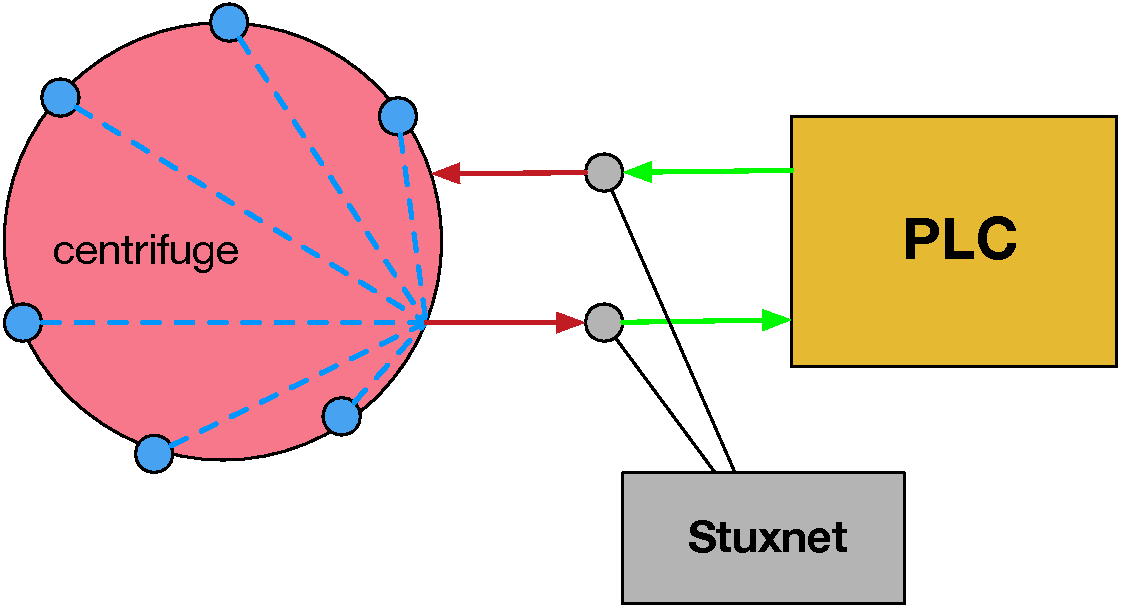
\includegraphics[width=.5\textwidth]{mim}},%
        {MITM attack carried out by Stuxnet: safe commands sent by the PLC (green) are replaced by dangerous ones (red); alarm readings from the centrifuge's sensors (red) are replaced by  safe ones\label{fig:stuxnet}}]
The behavior of Stuxnet's MITM component is outlined in Figure \ref{fig:stuxnet}. Its component operates by intercepting the commands sent by a PLC to a connected centrifuge. The malware first increased the speed of the centrifuge above normal levels for a short amount of time, and later slowed it down below normal levels for a longer period of time. It is believed that the resulting stress caused components of the centrifuge to expand and eventually destroy it. Under normal conditions, sensors installed in the centrifuge would have alerted the PLC---and its users---about the abnormal conditions, giving them a chance to shut down the system before damage occurred. However, as part of the MITM attack, Stuxnet also intercepted the sensor readings from the centrifuge, and sent to the PLC fake readings based on previous recordings that indicated that the system was operating normally (this is known as a \emph{replay attack}). 

A seriously concerning feature of MITM attacks is their ability to take control of the involved parties' inputs and outputs, making the attack virtually undetectable to the parties. In this section, we show that detection of a MITM attack is indeed possible if the detection task is reduced to that of reasoning about the truthfulness of a communication partner, as long as one has access to some external knowledge that can be used 
to evaluate
%as supporter or denial of 
the partner's statements.

To demonstrate this, we consider a simplified\ MITM attack scenario along the lines of Stuxnet's MITM component. For simplicity of presentation, we do not include in the scenario occurrences of actions, but it is not difficult to see that our approach extends in a natural way when actions occur.  %are present
\end{figwindow}


Consider the case of a motor, $M$, that can be \emph{on} or \emph{off.} A sensor mounted on the motor tells whether the motor is overheating (fluent $overheat$). A controller, $C$, is programmed to turn off the motor if it is found to be overheating.

Suppose now that the system is the target of a MITM attack. An attacker, $A$, manages to place itself between $C$ and $M$, intercepting the communications between them. $A$ intercepts the output of $M$'s sensor, discarding the sensor reading and always providing $C$ with a reading of $\neg overheat$ independently of the actual state of $M$, i.e, %. In doing so, 
the attacker could prevent $C$ from turning off an overheating motor, eventually causing it to be %come 
damaged. How can such an attack be detected?

The solution leverages a technique for reasoning about cyber-physical systems and their interaction with the physical environment discussed in \cite{nb15}. Suppose that a thermostat, $T$ is  located near the motor,  which generates an acoustic alert every $20$ minutes if the temperature of the room is above $90^\circ$F, in order to ensure that the operators take more frequent breaks. World knowledge furthermore tells us that, during a cold season, it is unlikely for the temperature in the room to be above $90^\circ$F.

The thermostat is not related to the functioning of the motor and, thus, it is conceivable that $A$ will not attempt to alter its activities.
However, given the proximity of the motor, an alert from the thermostat when the room is not hot can be taken as an indication that $M$ is indeed overheating (and that $M$'s sensor reading may have been tampered with). Let us see how one can draw this conclusion using our framework.

The relevant information can be formalized as follows:  %using the following statements:
{
\[
\begin{array}{l}
default(d_1^m, hot\_room, [alert]). \\
default(d_2^m, \neg hot\_room, [cold\_season]). \\
prefer(d_2^m,d_1^m, [ \: ]).\\
rule(r_1^m,cold\_season,[winter]). \\
default(d_3^m,overheat,[alert, \neg hot\_room]).
\end{array}
\]
}
Default $d_1^m$, says that, normally, an alert from $T$ indicates that the room is hot. Default $d_2^m$, states that, normally, the room is not hot during a cold season. The third statement expresses a preference for $d_2^m$ when both $d_1^m$ and $d_2^m$ are applicable. This captures the intuition that, during the cold season,  one will have a tendency to assume that the room is not hot even if an alert is heard. Rule $r_1^m$ encodes the world knowledge that winter is a cold season. Finally, the last statement says that, typically, if an alert is generated by $T$ when the room is not hot, then $M$ is overheating. The statement is encoded as a default to increase elaboration tolerance, making it possible, for example, to take into account faults in the thermostat or the presence of other heat sources.

Let us now suppose that we would like to evaluate the truthfulness of $M$'s sensor reading, and suppose that the sensor reports $\neg overheat$. The corresponding statement is:
$stm(\neg overheat,0).$
Next, an alert is generated by $T$:
$
obs(alert,1).
$
Let $KB_m$ be the corresponding knowledge base. Clearly, default $d_2^m$ is not applicable and $d_1^m$ leads us to conclude that the temperature in the room is above $90^\circ$F. Thus, the reasoner has no reason to doubt the sensor reading:
$
KB_{m} \models {+}stm(\neg overheat,0)@1.
$

Next, the system is informed that it is winter. The updated knowledge base, $KB_m'$, extends $KB_m$ by the statement:
$
obs(winter,2).
$
We have %Our framework now yields:
$
KB_m' \models {-}stm(\neg overheat,0)@2.
$
That is, the sensor reading from $M$ is deemed not truthful, which indicates that the system may be under a MITM attack.

\textcolor{red}{[REMOVE]} Finally, one can also reason about supporters and denials of $\neg overheat$. Given $KB_m$ and the above fluents, for example, it is not difficult to show that   $\emptyset$ is the minimal supporter  of $\neg overheat$ and $\{ winter \}$ is its minimal denial.
 
   
\section{Related Work }

%\memo{expand -- in addition with trust modeling, lp with preferences, default logic with preferences, cr-prolog} 

Within the scope of the ASP and logic programming community, this work is, to the best of our knowledge,  novel. As we have mentioned earlier, there is an extensive literature---within and outside the ASP community---for reasoning about actions and change, reasoning about defaults, and diagnostic reasoning about observations. All of these works are somewhat related to the proposed system. However, they are separate formalisms/systems that can be used as components of our system. In this sense, our work is related to    \cite{BalducciniG03b,BalducciniG03} and the ones mentioned earlier, such as \cite{brew99,BrewkaE00,DelgrandeST03,GelfondS98} as they are using ASP  in the implementation of a certain formalism. Also of note is that the proposed framework bears  similarity  to frameworks developed to
support \emph{diagnosis} as both rely on observations to draw conclusions but our framework 
does not focus on explaining what goes wrong and does not assume completeness of the 
knowledge of the agent (e.g., in the form of a complete
model).

Formalisms like ASP with preferences (e.g., \cite{Brewka05,BrewkaDRS15})  can provide a foundation for the implementation of the proposed framework---e.g., by 
facilitating the preferences between defaults.

%The work by \cite{BalducciniG03b} is related somewhat to our proposed implementation but only deals with observations and its extension \cite{BalducciniG03} includes an action theory but neither deals with a theory of defaults.     They are similar examples of separate formalisms for reasoning about observations or reasoning with defaults as mentioned earlier. 

The AI community has explored the issue of computational trust and reputation in several works---please see \cite{SabaterS05} for a survey. The survey focuses predominantly on trust models observed in multi-agent scenarios, taking explicitly into account the observations concerning interactions among agents. The survey provides classification of the models according to different dimensions: conceptual model (cognitive vs. game theoretical), information sources (direct interactions, direct observations, witness information, sociological information, prejudice), visibility (subjective vs. global), granularity (context dependent vs. non-context dependent), model type (trust vs. reputation), type of information exchanged (boolean vs. continuous), and agent behavior's assumptions (honest, biased but not lying, lying). Within such classification, our model focuses on trust---but could easily accommodate other interesting forms of reputation)---based on cognitive aspects, it builds on direct observations, but can accommodate sociological biases and prejudice through defaults, it captures subjective visibility, it is context dependent and relies on boolean information.
 
The survey in~\cite{ArtzG07} places a greater emphasis on surveying models of trust as models to predict attitude towards future interactions with an agent---with less emphasis on assessing the trustworthiness of a current statement.  

%\memo{need to work on -- to the conclusion 
%}
  
\iffalse  
 
\subsection{Relaxing Consequence} 
One of the advantages of using a declarative language like ASP is the ability
to explore alternative reasoning strategies. The proposed encoding is skeptical in 
the way it handles the assessment of statements---by considering a statement true when
supported by \emph{all} answer sets and false when its negation is supported by
all answer sets. There are variations of this approach that could be easily modeled. For example,
a trusting observe may want to accept the statement of the agent as long as this is not
explicitly contradicted.

\begin{definition}
Let $KB = \langle O, RD\rangle$ be a knowledge base and let us consider a statement 
$stm(l,s)$. We say that:
\begin{list}{$\bullet$}{\topsep=0pt \parsep=0pt \itemsep=0pt \leftmargin=10pt}
\item $KB \models {+}stm(l,s)@t$ if for every answer set $A$ of $KB$ we have that
        $h(\bar{l},t)\not\in A$;
\item $KB \models {-}stm(l,s)@t$ if every answer set $A$ of $KB$ contains
        $h(\bar{l},t)$;
\item the statement is otherwise unknown.
\end{list}
\end{definition}
This definition, applied to Example~\ref{ex2}, allows us to conclude:
  $KB_1 \models {+}stm(poor,0)@0$;
 $KB_1 \models   {-}stm(poor,0)@1$; and
 $KB_1 \models {+}stm(poor,0)@2$.
%
%\begin{list}{$\bullet$}{\topsep=1pt \parsep=0pt \itemsep=1pt}
%\item $KB_1 \models {+}stm(poor,0)@0$;
%
%\item $KB_1 \models   {-}stm(poor,0)@1$; and
%
%\item $KB_1 \models {+}stm(poor,0)@2$. 
%\end{list} 
   
\memo{
talk about time annotated knowledge bases, 
reputation evaluation, diagnosis} 
   
  
         
\subsection{Time-Annotated Knowledge Bases} 


The components of a knowledge base---as defined in the previous section---relate properties of the world at a single time instance. It is easy to imagine situations in which rules, defaults, and preferences could relate to information in different time points. For example, if the unit of time is months, the information ``if a graduate student fails the final examination, he/she needs to wait at least 1 year before re-taking the exam'' cannot be represented as a rule in the current framework since the relation between the fluent $take\_exam\_second\_time$ and the fluent $fail\_exam\_first\_time$  spans 12 units of times. 

We will next propose a generalization of the proposed framework, called 
\emph{time-annotated knowledge bases}, for dealing with the above issue. Let $l$ be a literal and $t$ be an integer. $l^t$ is called a \emph{time-annotated literal}. A \emph{time-annotated} rule, default, or preference has the form \eqref{rule}, \eqref{default}, or \eqref{pref}, respectively, whose $head$ and $body$ are now time-annotated literals and sets of time-annotated literals. For example, the relation between the two fluents $take\_exam\_second\_time$ ($ts$) and $fail\_exam\_first\_time$ ($ff$) can be represented by the set of rules: 
$$
\left \{ 
rule(exame\_time, (\neg ts)^i,  [ff^0])  
\mid i=1,\ldots,11 
\right\}
$$
 
Given a time-annotated knowledge base $KB$, the program $\Pi(KB)$ defined in the previous section can be easily modified for computing the truthfulness of statements. In fact, in all the rules of $\Pi(KB)$, $h(L, S)$ is replaced with $h(U, S+T)$ if $L$ is the time-annotated literal $U^S$. As an example, the rule~\eqref{lp:rule} becomes 

  \begin{equation}\label{lp:rule:tt}
\begin{array}{l}
h(H, S+T) \leftarrow  s(S),  
        rule(D, H^T, M),  \\ 
     \hspace{.1cm} N = \# count \{L^T : mem(M, L^T)\},  \\ 
    \hspace{.1cm}  \# count \{L^T : mem(M, L^T),  h(L, T{+}S) \} {==} N. 
      \end{array}
\end{equation} 


 
% \subsection{  Rules and Defaults} 

%Extending the language to allow time-dependent rules and defaults. Introducing time annotated literals: $l^t$ to denote $h(l, S+t)$. 
%
%\begin{align}
%rule(r, head^t, body) 
%\end{align} 

 
\subsection{A System for Reputation Evaluation}    
Given that reputation of agents is exhibited on what they say and what they do, the proposed framework can be used for evaluating agents' reputation if we have a rule (or a set of rules) for the evaluation, i.e., what does it mean for an agent to have excellent, good, or bad reputation. A reasonable rule for such a purpose could be devised using the ratio between the truthful and non-truthful statements made by agents, e.g., an agent has an excellent reputation if the ratio between her  truthful and non-truthful statements is 99\%. We note that this percentage is likely dependent on individual observer, the agent, and the application. For instance, it might be okay to classify a saleman as excellent if the percentage is 70\% but this thresthold would be insufficient for a doctor to be called as excellent. 

Given a knowledge base $KB$, a set of statements $S$ made by an agent, and a classification rule of the form ``an agent is of the type $xType$ if the ratio  between her  truthful and non-truthful statements is $y\%$,'' the program $\Pi_Q(KB)$ can be extended for determining whether or not the agent is of the type $xType$ in the following way. 

\begin{align} 
reputation(xType, T) \leftarrow s(T),\quad\quad  \label{rep} \\
NT = \#count \{L,T : \mathtt{t}(L, T)\},  \:\: \nonumber \\
NF =  \#count \{L,T : \mathtt{f}(L, T)\}, \nonumber \\
NT > 0, NT*100  \ge NF*y.        \quad\quad \:\: \nonumber
\end{align}     
where we assume that $y$ is given by an integer ranging between 0 and 100. 

Observe that this rule determines the reputation of the agent at the step $T$. The rule could be changed to compute the reputation of an agent over the full history considered by the program. Using the same method for computing the truthfulness of agents' statements, we can 
answer the question of whether or not the agent is of the type $xType$. 

Let $\Pi_R  = \Pi_Q  \cup \{\eqref{rep}\}$. If the program  
$\Pi_R   \cup \{\leftarrow \naf reputation(xType, t)\}$ has an answer set and the program 
$\Pi_R(KB)  \cup \{\leftarrow reputation(xType, t)\}$ has no answer set then we can conclude that the agent is of the type $xType$ 
at the time step $t$. 

\fi

%\memo{Discussing on different ways to deal with statement -- using information from other agents in evaluating truthfulness of other statements} 


%%%%%%%%%%%%%%%%%%%%%%%%%%%%%%%%%%%%%%%%%%%%%%%
\iffalse 
\begin{itemize} 
\item a \emph{conditional default} is of the form 
\begin{align}\label{c:default}
\alpha \Rightarrow default(d, head, body)
\end{align} 
where $d$ is the name of the default, $head$ is a fluent literal, and $body$ is a collection of literals.  A default \eqref{default} says that normally, if $body$ holds then $head$ also holds. 
\item a \emph{conditional preference} between two defaults is expressed by 
\begin{align}\label{c:prefs}
\alpha \Rightarrow prefer(d_1, d_2)
\end{align} 
where $d_1$ and $d_2$ are two default names. This says that $d_1$ is more preferred than $d_2$. 

\end{itemize} 

\subsection{Dealing with Inertial} 
 Rules for reasoning with inertial:
%
\begin{align}
ab\_inertial(H, \overline{H}, S) \leftarrow s(S), \label{lp:notinertial} \\
        app(D_1, H, S), \nonumber \\
        app(D_2, \overline{H}, S), \nonumber \\
        \naf defeated(D_1, H, S),  \nonumber \\
        \naf defeated(D_2, \overline{H}, S). \nonumber \\
h(H, S+1) \leftarrow s(S), h(H, S), \label{lp:inertial} \\ 
        \naf h(\overline{H}, S), \nonumber \\
        \naf ab\_inertial(H, \overline{H}, S). \nonumber        
\end{align} 
In the above rules, $ab\_inertial(H, \overline{H}, S)$ is an atom that indicates that 
The first rule, \eqref{lp:notinertial}, encodes our skepticism by defining the atom $not\_inertial(H, \overline{H}, S)$ w


%%%%%%%%%%%%%%%%%%%%%%%%%%%%%%%%%%%%%%%%%%%%%%% 

\subsection{Final Remark}
Let us conclude with a final remark. 
 The proposed framework bears  similarity  to the ASP frameworks developed to
 support \emph{diagnosis}. In particular, both frameworks  focus on using observations (and an underlying logical theory) to infer the correctness of some entity---a statement in our framework, a system in the case of diagnosis. 
 On the other hand, there is a profound difference between the two frameworks: unlike diagnosis, our 
 framework does  not rely on  a well elaborated theory of how the agent works. In particular, our frameworks 
 does not make any assumption about completeness of knowledge of the agent (e.g., in the form of a complete
 model).
  \fi 
   
 \section{Conclusions and Future Work}
In this paper, we proposed a general framework for reasoning about the truthfulness of statements
made by an agent. We showed how the framework can be implemented using ASP using well-known methodologies for reasoning about actions and change and for default reasoning with preferences. The framework does not assume complete knowledge about the agent being observed and the reasoning 
process builds on observations about the state of the world and occurrences of actions. We explored the use of the
framework in simple scenarios derived from man-in-the-middle attacks and  placed the proposed framework in the context of other related work.


The proposed work can be extended in several directions. First, the default theory considered in this paper is static in the sense that its rules and defaults encode knowledge about the world at a single time point. It is not difficult to imagine that rules and defaults can related knowledge at different time points (e.g., the knowledge about the behavior of some machine within a time interval). 
Second, we note that our implementation is rather impartial to statements by others (the ({\bf SK}) principle). An alternative view of this is to believe in every statement unless it is proven false. Third, it is reasonable to assume that there might be several sources of information that a user can employ to collect observations which include the agents that are observed. The reliability of each source might influence our decision on whether or not a statement could be believed as true. We believe that a combination of a model of trust together with attitude of agents as described in \cite{SabaterS05,ArtzG07} and our framework might be useful here. 
Our  system can be easily extended to deal with the first extension 
as it currently deals with time stamped literals already. The second extension might require the change in Def.~\ref{kb:entail}. The third extension might involve a significant amount of modification. We leave all these extensions for future work.  



\bibliographystyle{acmtrans}
\bibliography{enrico,bibfile,bib2010}

\end{document} 
